\chapter{Related Technologies}

The software was developed using both Java and \CPP{} while using multiple
open-source technologies. These technologies include:

\begin{itemize}
  \item Eclipse Modeling Framework
  \item EMF-IncQuery
  \item XText
\end{itemize}

The aim of this chapter is to familiarize the reader with these technologies.

%----------------------------------------------------------------------------
\section{Eclipse Modeling Framework}\label{sec:EMF}
%----------------------------------------------------------------------------

\emph{Eclipse Modeling Framework} (from now on referred to as \emph{\EMF{}}) is
a \Java{} based modeling tool and code generation facility for building applications based
on structured models. The specification of the model is written in \emph{XML
Metadata Interchange} (\emph{XMI}), which is an \emph{OMG} standard for
exchanging XML based metadata. Using the tools provided by \EMF{}, it is
possible to generate \Java{} code and facilities from a model specification
written in XMI. The generated code contains \Java{} classes representing the
model elements while the facilities include a basic model editor.

To talk further about \EMF{} it is important to differentiate between two very
important modeling concept.

\begin{itemize}
  \item \emph{Metamodel} - a model of model, a basic description of all the
  types which can exist inside of the model based on the metamodel.
  \item \emph{Instance model} - a model based on a metamodel, containing
  instances of the types defined in the metamodel
\end{itemize}

\EMF{} uses \emph{ECore} as it's main modeling language, which is a partial but most commonly acknowledged implementation of the OMG's
\emph{MetaObject Facility} (MOF) standard. It is a metamodel describing how a
user defined metamodel, which is an instance model of ECore, should look. The
relationship of ECore, user defined metamodel and instance model of the user
defined metamodel is described in figure \figref{ECore-Metamodel-Rel}.

\begin{figure}[!ht]
\centering
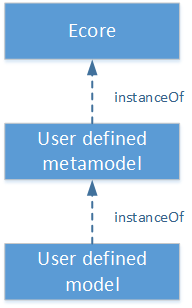
\includegraphics[width=40mm,keepaspectratio]{figures/ECore-Metamodel-Levels.png}
\caption{Different meta levels}
\label{fig:ECore-Metamodel-Rel}
\end{figure}

On the image it is clearly visible that the concepts metamodel and instance model
all depend on the perspective. From the perspective of ECore, ECore is a
metamodel while an ECore based user defined model is it's instance model. From
the perspective of the user defined metamodel, it is a metamodel, while it's
instance is an instance model.

The typical EMF workflow is to define a metamodel which describes the structured
data used in the application, generate the \Java{} code from it and then create
the data (instance model).

A metamodel is built using the following components (as described in ECore):

\begin{itemize}
  \item \emph{EClass} - Represents a class which can have attributes, references
  and operations. The instance model will consist of the instances of EClasses.
  \item \emph{EAttribute} - Describes an attribute which has a name and a type.
  For example an EClass can have an attribute \emph{Name} which has a type of
  \emph{String}.  
  \item \emph{EDataType} - Represents a user defined type. These are mostly used
  if none of the types described in ECore is suitable. EDataTypes allow for a
  mapping to simple \Java{} types.
  \item \emph{EReference} - Describes a relationship between two objects.
  Each reference has a name, a target EClass and a multiplicity. In addition
  there are multiple flags which can further customize the reference, from which
  the most important is the one called aggregation which decides whether this
  reference is a containment.
  \item \emph{EOperation} - These represent operations which can run on any
  instance of the containing EClass. These are sparsely used since they are
  cumbersome to work with.
  \item \emph{ESuperType} - Describes a parent-child relationship between two
  EClasses. This is the same as inheritance in object oriented programming
  languages.
\end{itemize}

The \EMF{} code generator is capable of generating the \Java{} classes from the
ECore model. Each Java class representing the EClasses defined in the ECore
model extends the EObject \EMF base class. This class provides a powerful
reflective API, with which it is possible to generically access the data of an
EClass instance without knowing it's type. In addition it is also possible to
register listeners for notification on model events, like a new model element
appearing, a model element disappearing or a property getting changed.

\subsection{Metamodel example}

The purpose of this section is to show an example of a metamodel. This
metamodel will be used in the examples later in the thesis. Figure
\figref{School_Metamodel} shows a metamodel that describes the structure of
schools.

\begin{figure}[!ht]
\centering
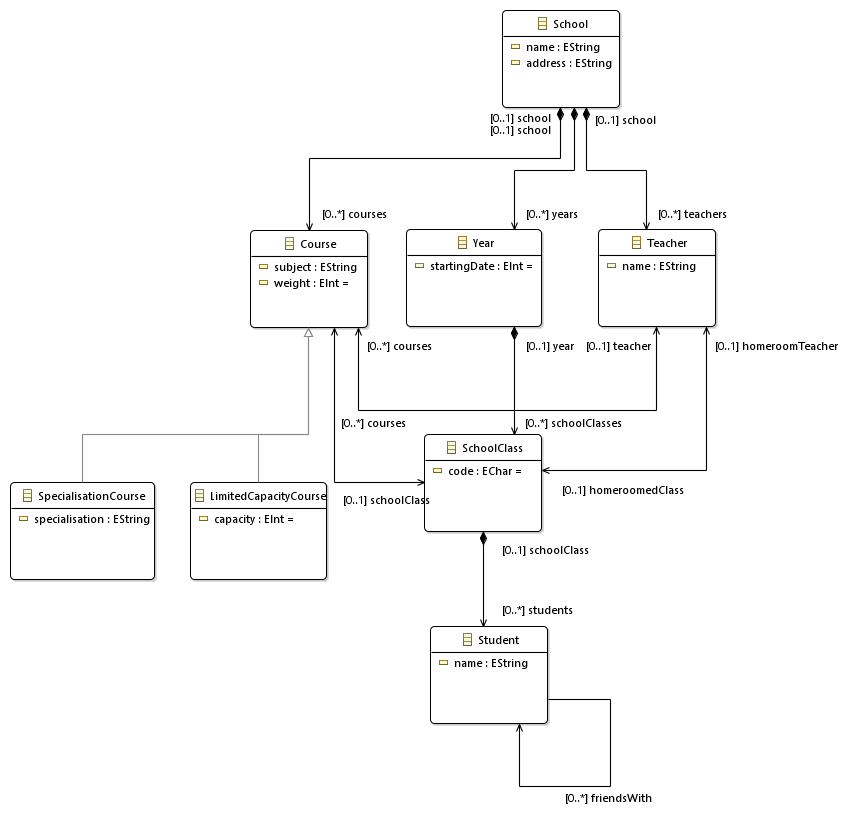
\includegraphics[width=133mm,keepaspectratio]{figures/school_class_diagram.png}
\caption{Metamodel of schools}
\label{fig:School_Metamodel}
\end{figure}

On the metamodel, some of the already explained parts of EMF can be seen. The
top element of the model, \emph{School} is an \emph{EClass}, while it's
\emph{name} is an \emph{EAttribute}. School has an \emph{EReference}
\emph{teachers} to the type \emph{Teacher} with a multiplicity of ``*''. This
EReference is a containment reference, marked by the small rhombus at the start
of the arrow. There is also an example of \emph{ESuperType} between
\emph{Course} and \emph{LimitedCapacityCourse}.

The root of the model is a school which has a name and an address. Each school
can have multiple teachers, years and courses. A year represents a school year,
has a starting date and contains several school classes. Each school class
has an identifying code and a single homeroom teacher, while each teacher can
only be the homeroom teacher of one class. A school class can have multiple
courses, while a course can only be taught to a single class. Each course has a
single teacher. A course can be either regular course which has a subject and a
weight, a specialization course which has a specialization in addition or a
limited capacity course which has a capacity. A school class has several
students and each students can have multiple friends. In the case of this
metamodel, most reference has an opposite reference, meaning it can be navigated in both directions.

\begin{figure}[!ht]
\centering
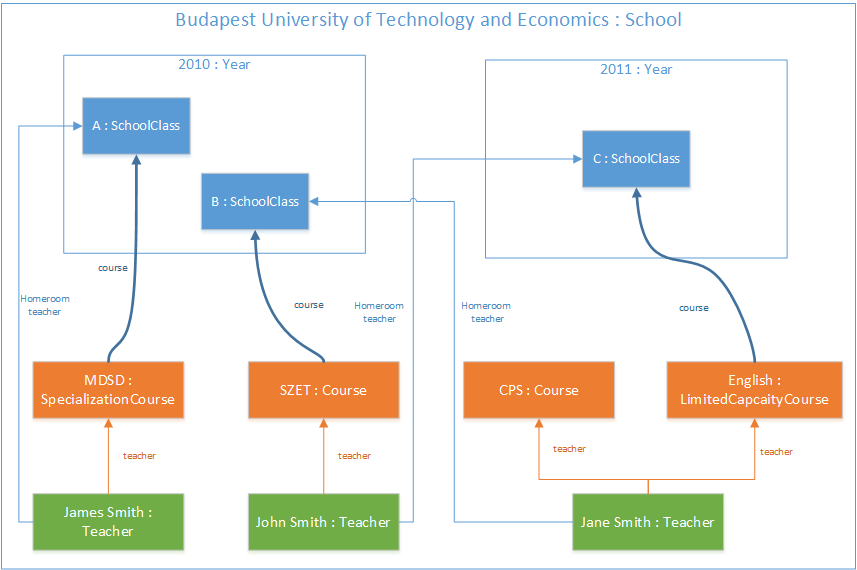
\includegraphics[width=133mm,keepaspectratio]{figures/InstanceModel.png}
\caption{A school instance model}
\label{fig:InstanceModel}
\end{figure}

Figure \figref{InstanceModel} depicts an instance model of the school metamodel.
The root of the model is a school instance with the name Budapest University of
Technology and Economics. It has two year instances, 2010 and 2011.
One year has 2 while the other has 1 school class. The school has 4 courses of
which one is a limited capacity course and another one is a specialization
course. Each course has a teacher and all of those teachers homeroom a class.

\pagebreak

Image \figref{InstanceModel_Eclipse} shows the same instance model, but as seen
inside the eclipse editor generated by EMF. The structure is clearly visible,
however the additional detail like references and attributes can not be
determined from it. There is a separate properties view that allows editing of
those information for the selected model element that is not shown on the
picture.

\begin{figure}[!ht]
\centering
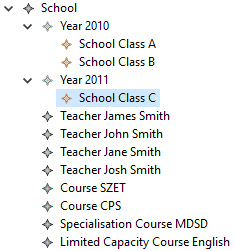
\includegraphics[width=50mm,keepaspectratio]{figures/InstanceModel_Eclipse.png}
\caption{A school instance model in eclipse}
\label{fig:InstanceModel_Eclipse}
\end{figure}

%----------------------------------------------------------------------------
\section{EMF-IncQuery}\label{sec:EMF-IncQuery}
%----------------------------------------------------------------------------

\emph{\EIQ{}} is a framework which allows for the execution of
\emph{declarative} queries over EMF models. These queries can be defined using
\EIQ{}'s own high level yet powerful query language. The main advantage of
the declarative query language is that it is not necessary to implement complex
model traversal algorithms in an imperative programming language (like \Java{})
to perform queries.

Queries defined via \EIQ{} can be easily tested development time, thanks to it's
rich tooling support. \EIQ{} generates \Java{} code for each
defined query which enables the user to run the queries over any EMF
instance model.

\subsection{The \EIQ{} Pattern Language}

The \EIQ Pattern Language is a high level, declarative graph pattern query
language. It has several advanced features of which this subsection of the
document will attempt to describe a few. All the examples will use the metamodel
shown on figure \figref{School_Metamodel}.

The following listing (\listref{SimpleIQPLExample}) shows the contents of a
simple \EIQ pattern definition file. The file begins with a package declaration
similar to \Java. The next line is an import, which imports the school metamodel
so \EIQ knows which metamodel is used.

The file has a single pattern definition named \emph{schools}. Each pattern
definition starts with the keyword \emph{pattern}, then has a name and by the
end has a parameter list. After these comes the pattern body. In this simple
case the pattern body simply declares that the parameter school has a type of
School, thus this pattern returns all school instance in a model.

\begin{lstlisting}[frame=single, language=IQPL,
label=listing:SimpleIQPLExample, caption=A simple query defined in \EIQ pattern
language]
package hu.bme.mit.cpp.localsearch.school.query

import "http://school.ecore"

pattern schools(school) {
	School(school);
}
\end{lstlisting}

The next listing (\listref{NavigationIQPLExample}) shows an example of a
navigation along a reference. In this case the results will be each
teacher-school pairs where the teacher teaches at the school.

\begin{lstlisting}[frame=single, language=IQPL,
label=listing:NavigationIQPLExample, caption=An example of a query along
reference] 
pattern teachersOfSchool(teacher, school) {
	School.teachers(school, teacher); 
}
\end{lstlisting}

Listing \listref{PatternCallIQPLExample} shows examples of calling positive and
negative pattern calls. In this example \emph{coursesOfTeacher} is called in a
positive manner from \emph{classesOfTeacher}. This basicly means copying the
body of \emph{coursesOfTeacher} in \emph{classesOfTeacher} while switching the
internal parameters to the local ones. The third pattern,
\emph{teacherWithoutClass}, uses negative pattern call, which means the called
pattern must not have a match with the provided parameters.

\begin{lstlisting}[frame=single, language=IQPL,
label=listing:PatternCallIQPLExample, caption=Pattern call example] 
pattern coursesOfTeacher(teacher, course) {
	Teacher.courses(teacher, course);
}

pattern specializationCoursesOfTeacher(teacher, course) {
	Teacher.courses(teacher, course);
	SpecializationCourse(course);
}  
 
pattern classesOfTeacher(teacher, schoolCourse) {
	find coursesOfTeacher(teacher, course);
	Course.schoolClass(course, schoolCourse);
}
 
pattern teacherWithoutSpecializationCourse(teacher) {
	neg find specializationCoursesOfTeacher(teacher, schoolCourse); 	
}
\end{lstlisting}

The following listing (\listref{AdvancedIQPLExamples}) shows examples to some of
the advanced pattern language features. The first query shows the usage of check
expressions. These allow simple Java-like expressions resulting in a boolean to
run within a query. The second pattern is an example of a disjunction where if
one of the bodies match the model that means a valid result.

\begin{lstlisting}[frame=single, language=IQPL,
label=listing:AdvancedIQPLExamples, caption=Advanced queries] 
pattern courseWithNameLongerThanWeight(course) {
	Course.subject(course, name);
	Course.weight(course, weight);
	check(name.length > weight); 
}

pattern friendlyTo(student1, student2) {
	Student.friendsWith(student1, student2);
} or {
	Student.friendsWith(student2, student1);
}
\end{lstlisting}

There are some more advanced features of the query language which I will not
detail like transitive closures and match counting, since they will not be
relevant.

\subsection{\EIQ{} API}

\EIQ{} provides an easy to use API to use the queries defined using the pattern
language. The API consists of classes provided by \EIQ{} and the generated code.
For each pattern definition, the following classes will be generated:

\begin{itemize}
  \item \emph{Match} - Represents a match for a specific query. A match contains
  references to elements from the queried model that match the current query.
  It is also possible to create a partial Match, where the user defines part of
  the references. This can be used to run \emph{bound} queries, which searches
  for matching patterns while taking into account the user defined elements.
  \item \emph{Matcher} - One of the most important classes, it starts the
  pattern matching of a specific query definition. The results of a pattern
  match can also be accessed through this class, while it also provides
  different views over the results.
  \item \emph{Processor} - This is an abstract helper class with a
  \emph{process} method. A user implemented MatchProcessor can be passed to a
  Matcher, which will call the process method using each match as a parameter.
  \item \emph{Evaluator} - These classes are helper classes to evaluate checks,
  they should not be used by the user.
  \item \emph{QuerySpecification} - The specification of a query which can also
  instantiate a matcher.
\end{itemize}

Listing \listref{EIQApiUsage} shows example of using the \EIQ{} API. The first
step is to create an \emph{EMFScope} from the EMF instance model. This is a
simple wrapper over anything that can be considered an EMF model. The next step
is to initialize an \emph{IncQueryEngine} over the newly created scope. After
this a \emph{Matcher} can be asked from the engine using the patterns
\emph{QuerySpecification}. The matcher allows the usage of a \emph{Processor} to
process each match. In this case, every schools name will get printed out on the
console.

\begin{lstlisting}[frame=single, language=Java,
label=listing:EIQApiUsage, caption=Usage of the \EIQ{} API] 
IncQueryEngine engine = IncQueryEngine.on(new EMFScope(model));

SchoolMatcher matcher = engine.getMatcher(SchoolQuerySpecification.instance);

matcher.forEachMatch(new SchoolsProcessor() {
	@Override
	public void process(final School school) {
		System.out.println(school.getName());
	}
});
\end{lstlisting}

%----------------------------------------------------------------------------
\section{Xtend}\label{sec:Xtend}
%----------------------------------------------------------------------------

Xtend is a statically typed dialect of \Java{} which compiles into human
readable \Java{} code. The language has it's roots in \Java{} but improves on
many aspects of it:

\begin{itemize}
  \item \emph{Extension methods} - allows adding new methods to closed types
  without modifying them
  \item \emph{Lambda expression} - Lambda expression is a code snippet wrapped
  in an object that can be passed around easily. This was a more important
  feature before \Java 8 since it allowed a more concise way of passing around
  methods (instead of anonymous classes), but it still improves over \Java 8
  lambdas since they can be used in place of abstract classes, not only
  functional interfaces.
  \item \emph{Active annotations} - Using active annotations, the \Java code
  compilation can be customized.
  \item \emph{Template expression} - These allow easy parametrization of
  strings. This feature is most useful for generating code.
  \item \emph{Type inference} - Xtend can usually infer the types of variables,
  methods thus reducing code size (especially in case of generics).
  \item \emph{Properties} - Xtend interprets setters and getters as properties,
  which makes accessing and writing properties of classes less cumbersome since
  they can be accessed by their name (i.e., instead of calling
  obj.getName() one can access name using obj.name).
  \item \emph{Operator overloading} - In Xtend it is possible to overload
  operators for any type. It is mostly useful for mathematical computations with
  BigInteger or when writing math library using vectors and matrices.
\end{itemize}

Since Xtend compiles to \Java code there is no interoperability issue between
\Java libraries and Xtend code or vice versa.

\subsection{Xtend example}

For introduction, listing \listref{XtendIntro} shows the previous \EIQ API usage
example code (\listref{EIQApiUsage}) translated to XTend. There are several
small differences like static access is done through ``::``, no ``;'' at end of
line or using ``val'' instead of type, but the most significant difference is
the usage of lambda expression in \emph{forEachMatch}. In this case, the lambda
expressions parameter is a \emph{SchoolMatch} that has a school property. In
lambda expressions if they only have a single parameter, then the parameter's
scope is accessible in the local scope, so basically it is possible to access
school without writing out the parameters name and the dot. It is also notable
that properties can be accessed directly, there is no need to write getName().

\begin{lstlisting}[frame=single, language=Xtend,
label=listing:XtendIntro, caption=Usage of the \EIQ{} API with Xtend] 
val engine = IncQueryEngine::on(new EMFScope(model))

val matcher = engine.getMatcher(SchoolQuerySpecification::instance)

matcher.forEachMatch[println(school.name)]
\end{lstlisting}

Xtends most important feature in my case was it's code generation capability
through template expressions, to which listing \listref{XtendCodeGen} gives an
example. This example generates a simple \CPP{} program which prints out a
greeting. The most important things are how the string between the tripple ticks
maintains it's identation and how easy it is to parametrize the text.

\begin{lstlisting}[frame=single, language=Xtend,
label=listing:XtendCodeGen, caption=Xtend code generation] 
def genCppGreeting(String... names) ```
	#include <iostream>

	int main(int, char**) {
		�FOR name : names�
		std::cout << "Hello �name�!" << std::endl;
		�ENDFOR�
	}
```
\end{lstlisting}